\section{File System Implementation}
\subsection*{File Block Allocation}
\emph{Contiguous:} (+) Simple to keep track(start \#+length), fast access. (-) external fragmenation, specify file size in advance.\\
\emph{Linked List:} Store file start end. (+) No fragmentation. (-) slow random access(disk speed pointer), part of block used for pointer.\\
\emph{Linked List V2.0:} Move all block pointers to File Allocation Table(FAT)(in memory). (+) Faster random access(traversal in memory). (-) FAT size depends on disk size, consumes memory.\\
\emph{Indexed allocation:} Linked scheme(linked list of index blocks), multilevel index(1st lvl index block points to several 2nd level index blocks), combined scheme.

\subsection*{Free Space Management}
Linked list(linked indexed representation), array(compress to bitmap).\\
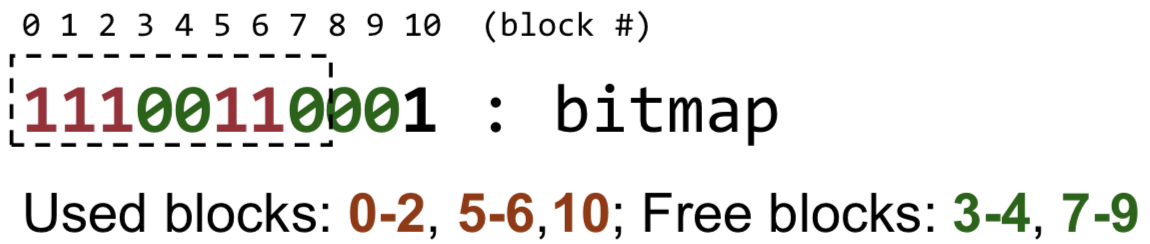
\includegraphics[width=0.75\linewidth]{images/bitmap-free-block}

\subsection*{MSDOS}
FAT stored in disk, duplicated in RAM. FAT16 has root dir size limit of 512 entries.\\
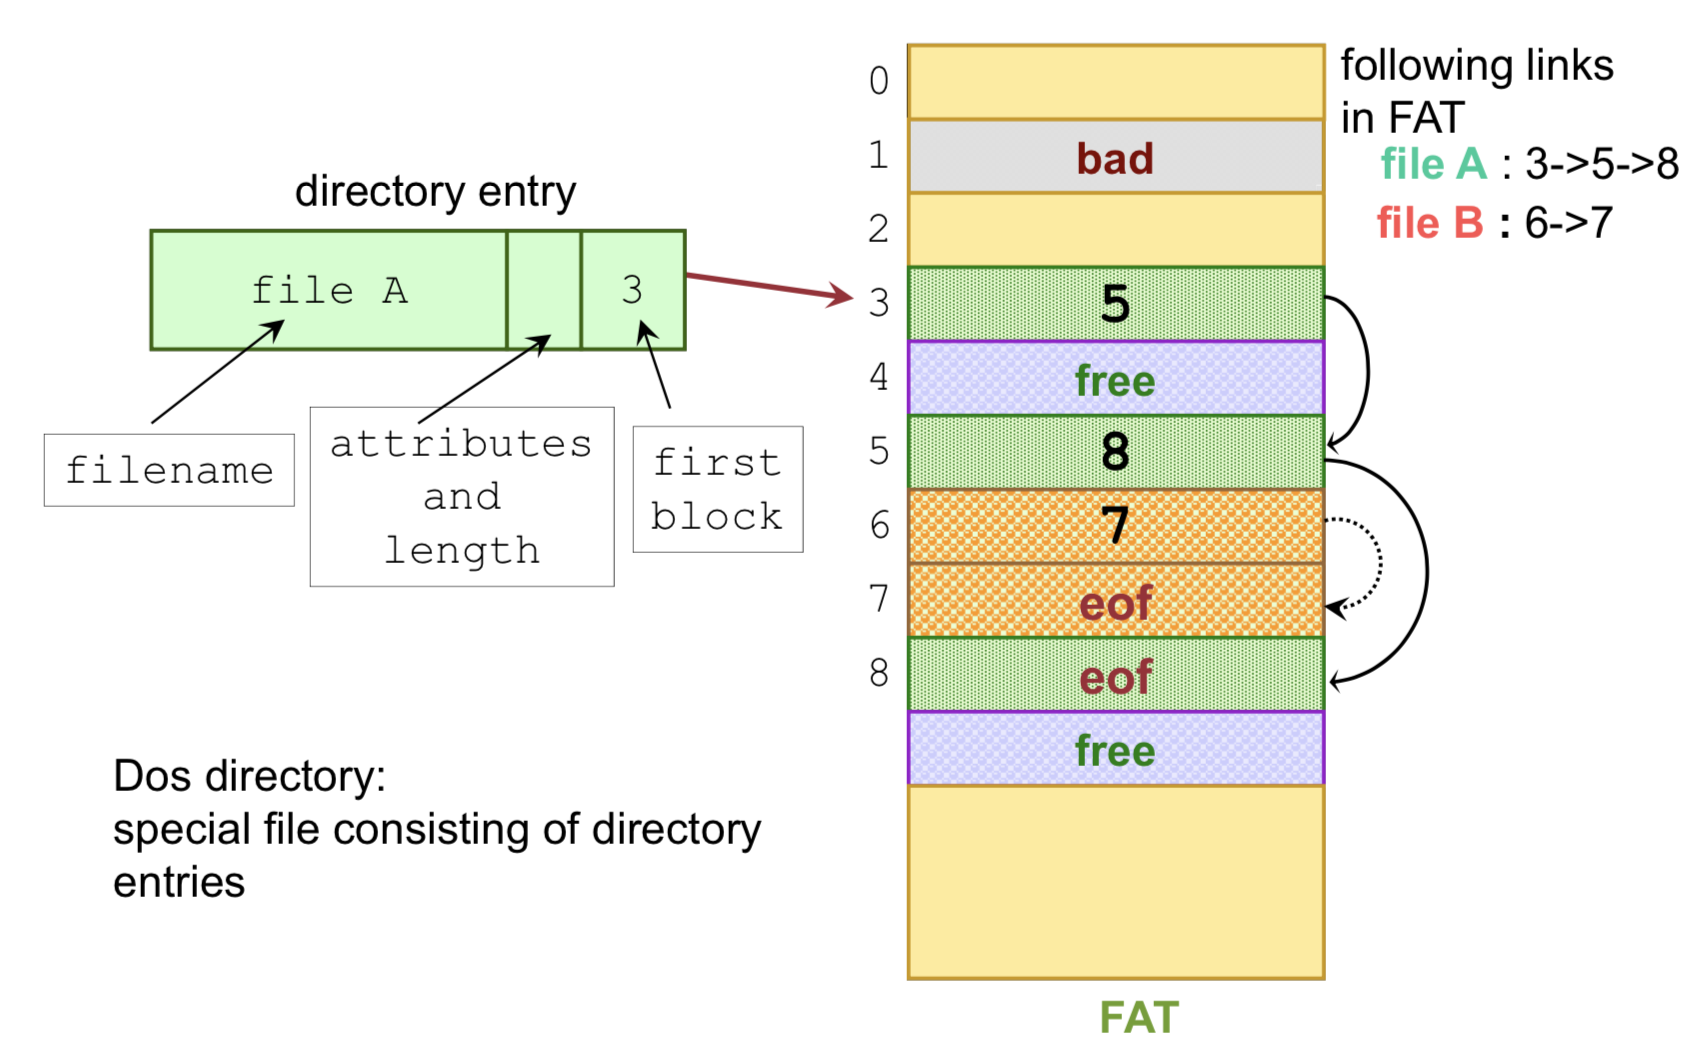
\includegraphics[width=0.9\linewidth]{images/msdos-fat}\\
\emph{Deleting file:} Set first letter in filename to 0xE5, set FAT entries in linked list to FREE.\\
\emph{Cluster:} 16 bits numbers in FAT entries, logical block size=cluster size=multiple of sectors. Large cluster size -> large internal fragmenation.\\
\emph{Disk Fragmenation:} logical contiguous blocks far apart on disk(about time). FAT: less disk fragmentation with large cluster size, solution: run defragmentation(compaction) on entire FS. s5fs: worse since smaller logical block size.

\subsection*{Unix s5fs}
\emph{Inode:} actual file object, one per file. Contains: reference count for hard links, Table of Contents(TOC) mapping file data to disk blocks(hybrid multi-lvl index).\\
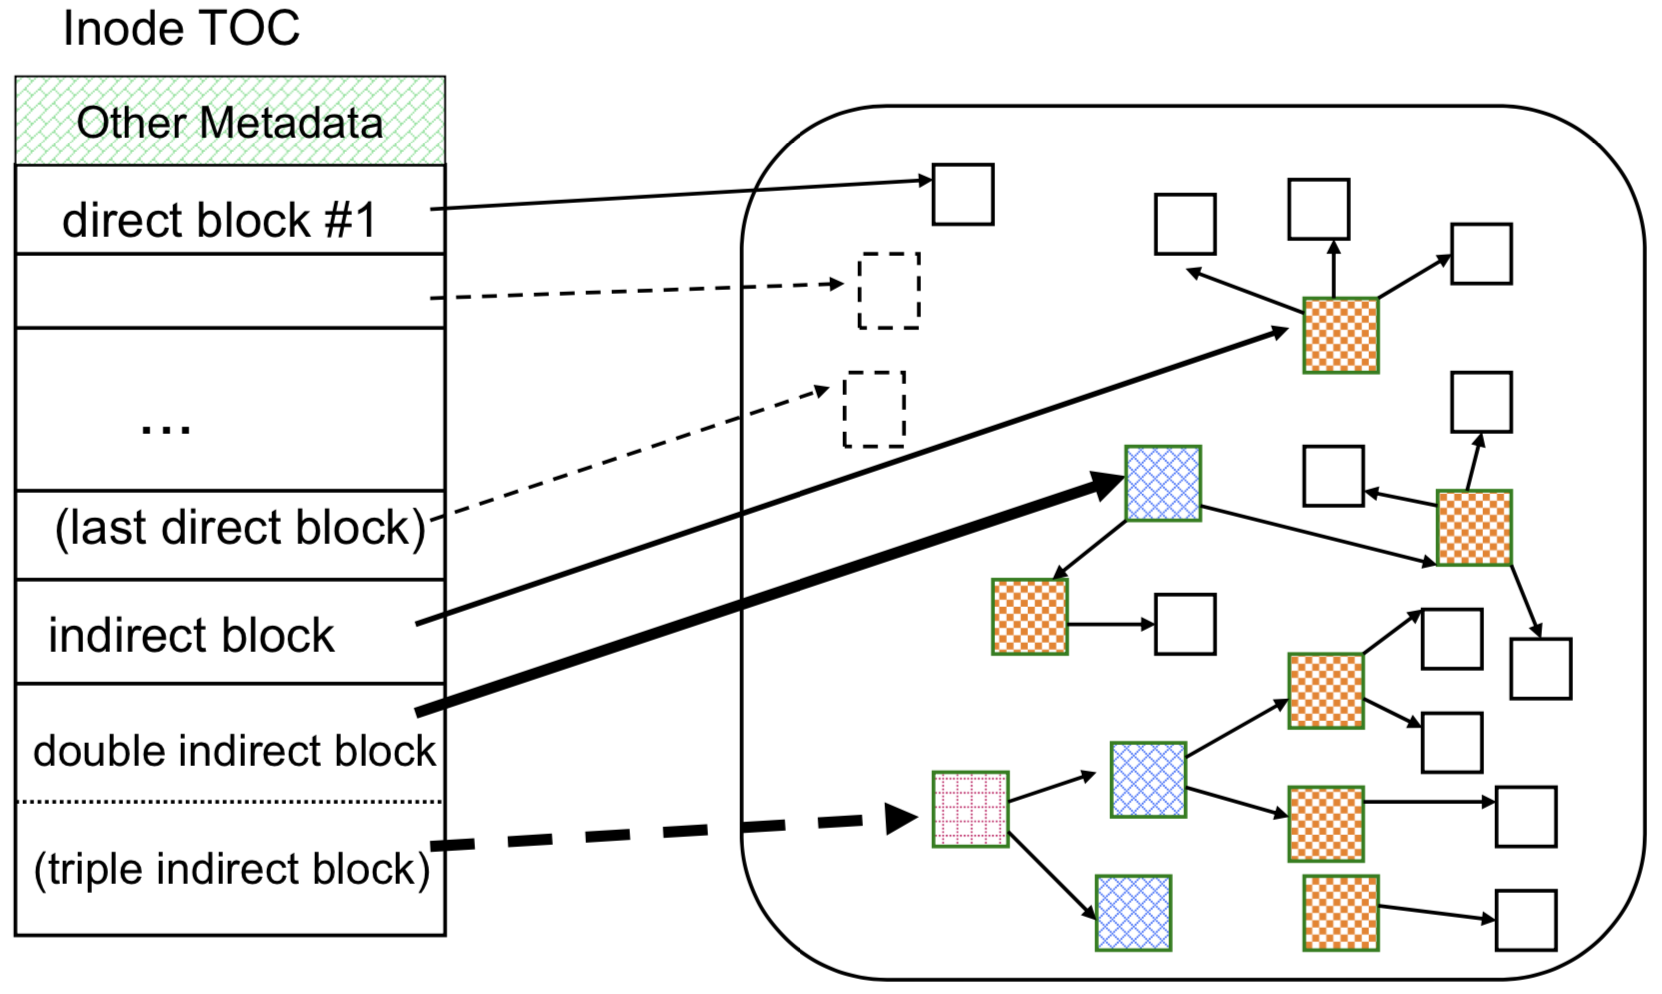
\includegraphics[width=0.9\linewidth]{images/s5fs-toc}\\
Allow blocks which do not exist(logical zero filled holes) - set block pointer to NULL in TOC, return zeroes when read.\\
\emph{Directories:} Map inode \# to filename. Array of 16-byte entries(inode 16 bits, filename 14 bytes). Deleted file has inode 0.\\
\emph{Hard links:} same file to have more than one filename(create DAG). ln. Same inode \# for different filenames. Remove reference with unlink() syscall. Deleting: remove dir entry, decre inode link count, free file object when link count=0.\\
\emph{Caching:} add a buffer cache in memory for disk blocks. Write can be faster than reads(can write to buffer). Use LRU to replace blocks in cache. sync(2) syscall requests dirty buffers be flushed, fsync(2) waits for completion.